\documentclass[11pt]{article}

% ── Layout & typography ─────────────────────────────────────────────────
\usepackage[margin=2.2cm]{geometry}
\usepackage[T1]{fontenc}
\usepackage[utf8]{inputenc}
\usepackage{lmodern}
\usepackage{microtype}
\usepackage{setspace}\setstretch{1.15}
\usepackage{parskip}
\usepackage{lineno}\linenumbers
\usepackage[font=small,labelfont=bf]{caption}
\setlength{\emergencystretch}{2em}

% ── Math, figures, references ──────────────────────────────────────────
\usepackage{amsmath}
\usepackage{amssymb}
\usepackage{graphicx}
\usepackage{subcaption}
\usepackage{comment}
\usepackage{url}
\usepackage{xcolor}
\usepackage[colorlinks=true, allcolors=blue!50!black, citecolor=teal!60!black]{hyperref}
\usepackage[
    backend=bibtex,
    style=authoryear,
    sorting=nyt,
    natbib=true
]{biblatex}
\addbibresource{references.bib}

\title{\sffamily\bfseries How predictable is precipitation from the resolved
large-scale state?\\[4pt]
{\large\mdseries A scale-dependent information horizon}}

\author{
Tim Zhou$^{1}$, \quad Sophie Abramian$^{2}$, \quad Sara Shamekh$^{1}$ \\[5pt]
\small $^{1}$Courant Institute of Mathematical Sciences, New York University \\
\small $^{2}$Columbia University
}
\date{\today}

\begin{document}
\maketitle

\begin{abstract}
\noindent
Increasing model resolution is widely equated with increasing forecast skill,
yet resolving a convective cell does not make it predictable: resolution
controls what a model can \emph{represent}, not what the atmosphere will
\emph{do}. Parameterised convection makes precipitation a deterministic
function of the resolved state, hiding a stochasticity that
convection-permitting models expose. We ask how much predictive information the resolved large-scale state carries
about precipitation --- at what spatial scale, and out to what lead time ---
a property of the atmosphere that upper-bounds any deterministic forecast system. Using a global convection-permitting
simulation (DYAMOND/MPAS, $3.8$\,km) as truth, we train per-lead neural
networks as best-case estimators of the state-to-precipitation map, and
evaluate them with an object-based decomposition that separates the
precipitation error into \emph{detection} (trigger), \emph{area}, and
\emph{intensity} (amplitude). Detection skill collapses monotonically with
decreasing system scale, and an exponential fit yields a conditional
predictability horizon for the convective \emph{trigger} of only
$T_e\!\approx\!0.7$\,h at scales below $65$\,km, rising to $\sim$9\,h for
systems larger than $200$\,km. For large systems the \emph{amplitude} remains
informative for many hours ($T_e\!\approx\!21$\,h), while for small systems
amplitude fades as rapidly as the trigger. The only small-scale signal that
survives the trigger horizon is the externally forced diurnal cycle: the
network stores this forced climatology in its weights and reinjects it even
when all solar-tied inputs are removed --- substituting climatology for
forecast skill once predictability is lost. The same scale-dependent collapse
appears in GraphCast, an operational AI model of entirely different
architecture and training data, indicating a physical, architecture-independent
bound on data-driven precipitation forecasting at convective scales.
\end{abstract}

\section{Introduction}

Precipitation predictability spans many orders of magnitude in space and time.
A squall line can be warned a day ahead; a single convective cell cannot be
warned hours ahead. Both facts are widely accepted, yet the precise boundary
between them --- at what spatial scale and lead time the resolved large-scale
atmospheric state loses its grip on precipitation --- remains poorly quantified.
The question is not merely academic: flash floods, isolated heavy rainfall, and
convective wind damage cluster at the small end of the scale spectrum, where
predictability is shortest and warning lead times matter most.

A fundamental obstacle is a widespread modelling artefact.
In coarse-resolution numerical weather prediction, convection is parameterised:
precipitation becomes a deterministic function of the resolved state, so
coarse-model rain inherits the long predictability of the large-scale flow.
Global convection-permitting models (CPMs), now routinely run at $3$--$4$\,km
\citep{satoh2019global, stevens2019dyamond}, remove this scheme and let the
resolved environment produce many possible realisations of where and when cells
fire, recovering the atmosphere's true, scale-dependent predictability limit
\citep{lorenz1969predictability, zhang2007mesoscale, judt2018insights,
hohenegger2007predictability}.
Increasing horizontal resolution is routinely equated with increasing forecast
skill; for precipitation at convective scales, this equation fails, because
resolution determines what a model can \emph{represent}, not what the
atmosphere will \emph{do}.

Quantifying that limit requires a verification framework that separates
distinct failure modes.
Standard pixel-wise scores --- RMSE, equitable threat score, correlation ---
apply a double penalty to a displaced precipitating system (it scores as
both a miss and a false alarm) and reward spatial smoothing, suppressing the
small-scale features that are hardest to predict \citep{gilleland2009}.
Object-based methods instead match precipitating systems and independently
score their detection, area, and intensity \citep{davis2006}.
Such a decomposition separates the \emph{trigger} failure (wrong location or
missed initiation, governed by sub-grid boundary-layer processes that are
effectively stochastic at the resolved scale) from the \emph{amplitude}
failure (correct location, wrong intensity, governed by large-scale
thermodynamics that evolve on the timescale of the flow).
These two failures have different physical origins and, as we show, very
different predictability timescales.

Data-driven weather models have recently achieved forecast skill competitive
with operational NWP for large-scale variables at multi-day leads
\citep{lam2023graphcast}, yet precipitation remains a known challenge at
convective scales \citep{ravuri2021}.
A neural network trained to minimise mean squared error against a CPM truth
predicts the conditional mean of the precipitation distribution --- a quantity
that is necessarily blurred when the distribution is broad and triggering is
stochastic.
Understanding whether a given model \emph{cannot} predict small-scale rain, or
whether no deterministic model \emph{can}, requires separating architectural
limitations from physical ones.

Against this background we address three questions:
\begin{enumerate}
  \item \emph{How much predictive information does the resolved large-scale state
        carry about precipitation, and how does this depend on system scale and
        on the choice of input variables?}
        We use zero-lead networks as instruments that quantify how much
        instantaneous environmental information the state carries about rain,
        and compare predictor sets to isolate the contribution of dynamical
        versus thermodynamic variables.
  \item \emph{How rapidly does this predictive information decay with lead time,
        and is the decay rate scale-dependent?}
        We fit an exponential information horizon separately for trigger
        (detection) and amplitude (intensity) skill across scale bands.
  \item \emph{Is the observed scale-dependent collapse specific to our network,
        or is it a physical, architecture-independent bound?}
        We apply the same decomposition to GraphCast, a state-of-the-art AI
        forecast model trained on entirely different data with a different
        architecture.
\end{enumerate}

Section~\ref{sec:methods} describes the data, the lead-conditioned network, and
the object-based decomposition metric.
Results are presented in Section~\ref{sec:results}: network performance and
variable sensitivity at zero lead (\S\ref{sec:lead0}), the scale-dependent
predictability horizon (\S\ref{sec:horizon}), and the generalisation to
GraphCast (\S\ref{sec:graphcast}).
Section~\ref{sec:discussion} discusses physical interpretation, the role of the
forced diurnal cycle as a learned climatological prior, and implications for AI
precipitation forecasting.
Section~\ref{sec:conclusion} concludes.

\section{Data and Methods}
\label{sec:methods}

\subsection{Data}
\label{sec:data}

The dataset is the DYAMOND MPAS-Atmosphere global cloud-resolving simulation,
performed at $\sim$3.8\,km horizontal resolution with 15-min output over a
40-day boreal-winter period.
MPAS employs a fully compressible, nonhydrostatic dynamical core on an
unstructured mesh, enabling explicit simulation of convective processes; cloud
microphysics are represented with a double-moment scheme.
Global cloud-resolving models explicitly resolve deep convection and provide
dynamically consistent four-dimensional fields essential for process-level study
and data-driven modelling \citep{satoh2019global}.
MPAS generally reproduces mean precipitation and its diurnal cycle within the
multi-model DYAMOND range \citep{stevens2019dyamond}, though it tends to
overestimate deep convective clouds and heavy rainfall relative to the IMERG
satellite product \citep{feng2025mpas}.
All fields are regridded to a $0.25^\circ$ longitude--latitude grid and cropped
to the tropics ($\pm40^\circ$), retaining 15-min snapshots as individual samples.

\subsection{Lead-conditioned network}
\label{sec:net}

We frame the problem as follows.
Let $X(t)$ be the resolved large-scale state at time $t$ and $P_{t+\tau}$ the
precipitation field at lead $\tau$.
A network that minimises mean squared error over $P_{t+\tau}$ converges to
$\mathbb{E}[P_{t+\tau}\mid X(t)]$ --- the conditional mean, and the Bayes-optimal
deterministic predictor of precipitation given the resolved state.
We use this network as an \textbf{instrument}: its skill measures how much
predictive information the environment carries about the rain; its failure is
evidence of genuine physical unpredictability, not model weakness.

\paragraph{Input state.}
The full state $X(t)$ comprises nine variables spanning the radiative--moist
background and the dynamical structure: column water vapour (PW), $2$\,m
temperature ($T_{2m}$), outgoing longwave radiation (OLR), moist static energy
at $500$ and $850$\,hPa ($h_{500}$, $h_{850}$), and zonal and meridional winds
at $500$ and $850$\,hPa.
We compare this full nine-variable set against two reduced five-variable sets ---
thermodynamics only with moist static energy, and thermodynamics only with
relative humidity --- to isolate the contribution of the dynamical fields.

\paragraph{Architecture.}
The network is a 2-D U-Net with skip connections and bilinear upsampling
(base width $64$ channels, depth $5$, dropout $0.05$), trained on
$64\times64$ patches tiled from the tropical crop.
It has a single softplus output head, enforcing $\widehat{P}\ge 0$.

\paragraph{Training objective.}
The network minimises mean squared error restricted to rain pixels,
\begin{equation}\label{eq:loss}
\mathcal{L} = \frac{1}{|\Omega|}\sum_{i\in\Omega}\!\bigl(\widehat{P}_i - P_i\bigr)^2,
\qquad \Omega = \{i : P_i > 0\},
\end{equation}
where the sum runs over all raining pixels in the batch. Masking to $\Omega$
prevents the heavy rain/no-rain class imbalance from suppressing predicted
intensities; the softplus output independently enforces non-negativity.
A \emph{separate} network is trained for each lead
$\tau\in\{0,0.25,0.5,0.75,1,1.5,2,3,4,6\}$\,h, removing autoregressive error
accumulation; the skill-versus-lead curve is a clean measurement of
state-to-rain predictability alone.

\subsection{Object-based precipitation decomposition}
\label{sec:objmethod}

We evaluate forecasts at the level of precipitating \emph{systems} rather than
grid points.
For a single 2-D field at one time we threshold at $r_0=0.1$\,mm\,h$^{-1}$ and
label connected components with 8-connectivity.
For each system we accumulate the precipitating area $A$ (km$^2$), the total
precipitation $P=\sum \mathrm{rate}\cdot\mathrm{area}$ (mm\,km$^2$), and the
area-weighted mean intensity $\rho=P/A$ (mm\,h$^{-1}$), with $L=\sqrt{A}$ as
the characteristic scale.
Defining $\rho$ as the area-weighted mean makes the identity exact,
\begin{equation}\label{eq:Prhoa}
P=\rho\,A,\qquad
\ln\!\frac{P_p}{P_t}=\underbrace{\ln\!\frac{A_p}{A_t}}_{\Delta\ln A}
+\underbrace{\ln\!\frac{\rho_p}{\rho_t}}_{\Delta\ln\rho},
\end{equation}
so the precipitation error of a matched system splits exactly into an \emph{area}
error $\Delta\ln A$ and an \emph{intensity} error $\Delta\ln\rho$, with no
cross-term.
The log form is scale-free, so a $+50\%$ area error on a $30$\,km cell and on a
$400$\,km complex contribute comparably.

\paragraph{Matching.}
Within each frame, predicted systems are matched to truth systems by greedy
descending intersection-over-union (IoU), accepting a pair when
$\mathrm{IoU}\ge0.1$.
This yields one-to-one matches and three roles: \emph{match} (truth+pred),
\emph{miss} (truth system with no predicted counterpart), and \emph{false alarm}
(predicted system with no truth counterpart).
A system that is displaced but still overlapping is a \emph{match} carrying
area/intensity error, not a miss--false-alarm pair: the matching tolerates
sub-system displacement, avoiding the double penalty of pixel-wise scores.

\paragraph{Skill metrics and predictability horizon.}
Stratified into log-spaced scale bins, we compute per bin the probability of
detection $\mathrm{POD}=n_{\text{match}}/(n_{\text{match}}+n_{\text{miss}})$,
the false-alarm ratio $\mathrm{FAR}=n_{\text{fa}}/(n_{\text{match}}+n_{\text{fa}})$,
and the precipitation-weighted area and intensity biases $\Delta\ln A$,
$\Delta\ln\rho$ for matched systems.
To summarise the decay of skill $\mathcal{S}(\tau)$ with lead we fit
\begin{equation}\label{eq:efold}
\mathcal{S}(\tau)\approx(\mathcal{S}_0-\mathcal{S}_\infty)\,e^{-\tau/T_e}+\mathcal{S}_\infty,
\end{equation}
yielding a zero-lead skill $\mathcal{S}_0$, an $e$-folding predictability
time $T_e$, and an asymptotic floor $\mathcal{S}_\infty$ set by
climatology or persistence.

\section{Results}
\label{sec:results}

\subsection{Network performance at zero lead and variable sensitivity}
\label{sec:lead0}

At zero lead, OLR directly tracks cloud-top temperature, PW reflects column
saturation, and $T_{2m}$ captures the boundary-layer thermodynamic state.
Zero-lead performance therefore measures how much predictive information the
resolved state carries about the current precipitation field --- an upper bound
on what any lead-$\tau$ network can achieve.

Figure~\ref{fig:tropicwide} shows the prediction at $3$\,h lead for context:
the network reproduces the large-scale organisation of precipitation --- the
ITCZ, major convective envelopes --- but is visibly smoother than the truth,
with the difference field dominated by small-scale structure.
This smoothing is expected: when triggering is stochastic, the conditional mean
is a spatial average over all possible realisations of where cells could fire.

The object-based decomposition on a single mid-afternoon scene over West Africa
(Fig.~\ref{fig:method}) makes the failure mode concrete: the model captures
large organised convective bands but is blind to the scatter of small
($\lesssim50$\,km) cells along the ITCZ, which are missed rather than displaced.

\begin{figure}[t]
\centering
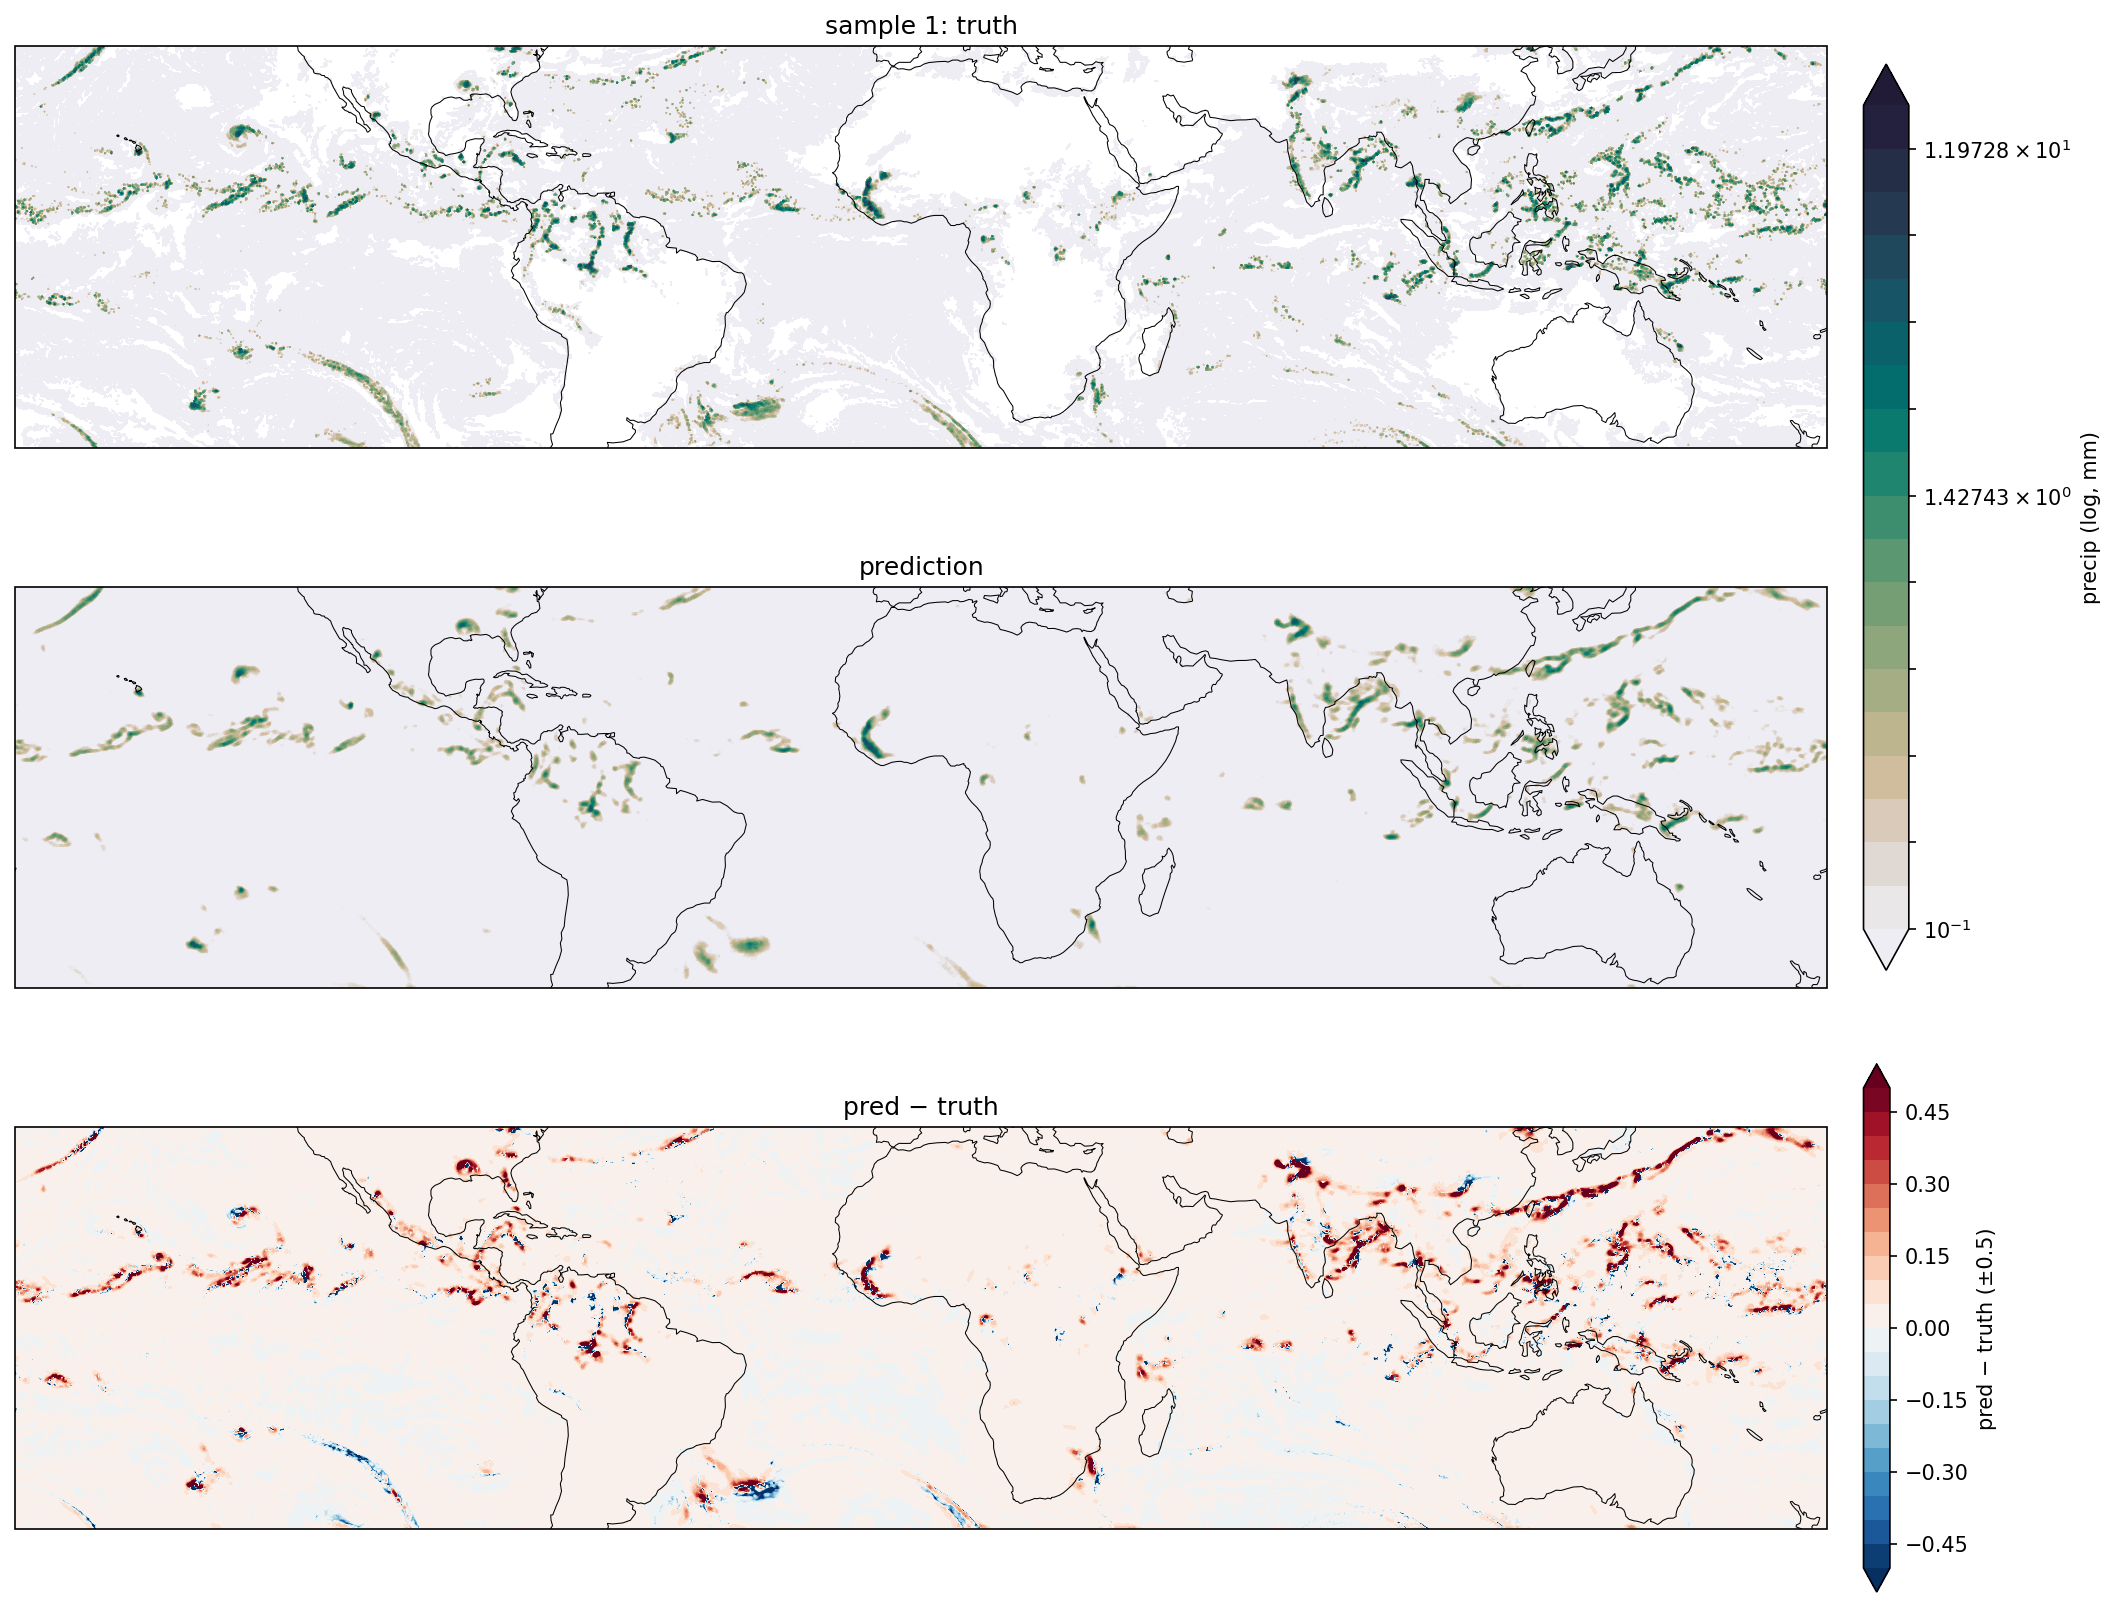
\includegraphics[width=\textwidth]{figures/tropicwide_truth_pred_diff_lead3h.png}
\caption{Tropic-wide precipitation at $3$\,h lead: truth (left), prediction
(centre), and difference (right) for one held-out test frame. The prediction
captures the large-scale organisation but is smoother than the truth; the
difference field is dominated by displaced and under-predicted small-scale
features.}
\label{fig:tropicwide}
\end{figure}

\begin{figure}[t]
\centering
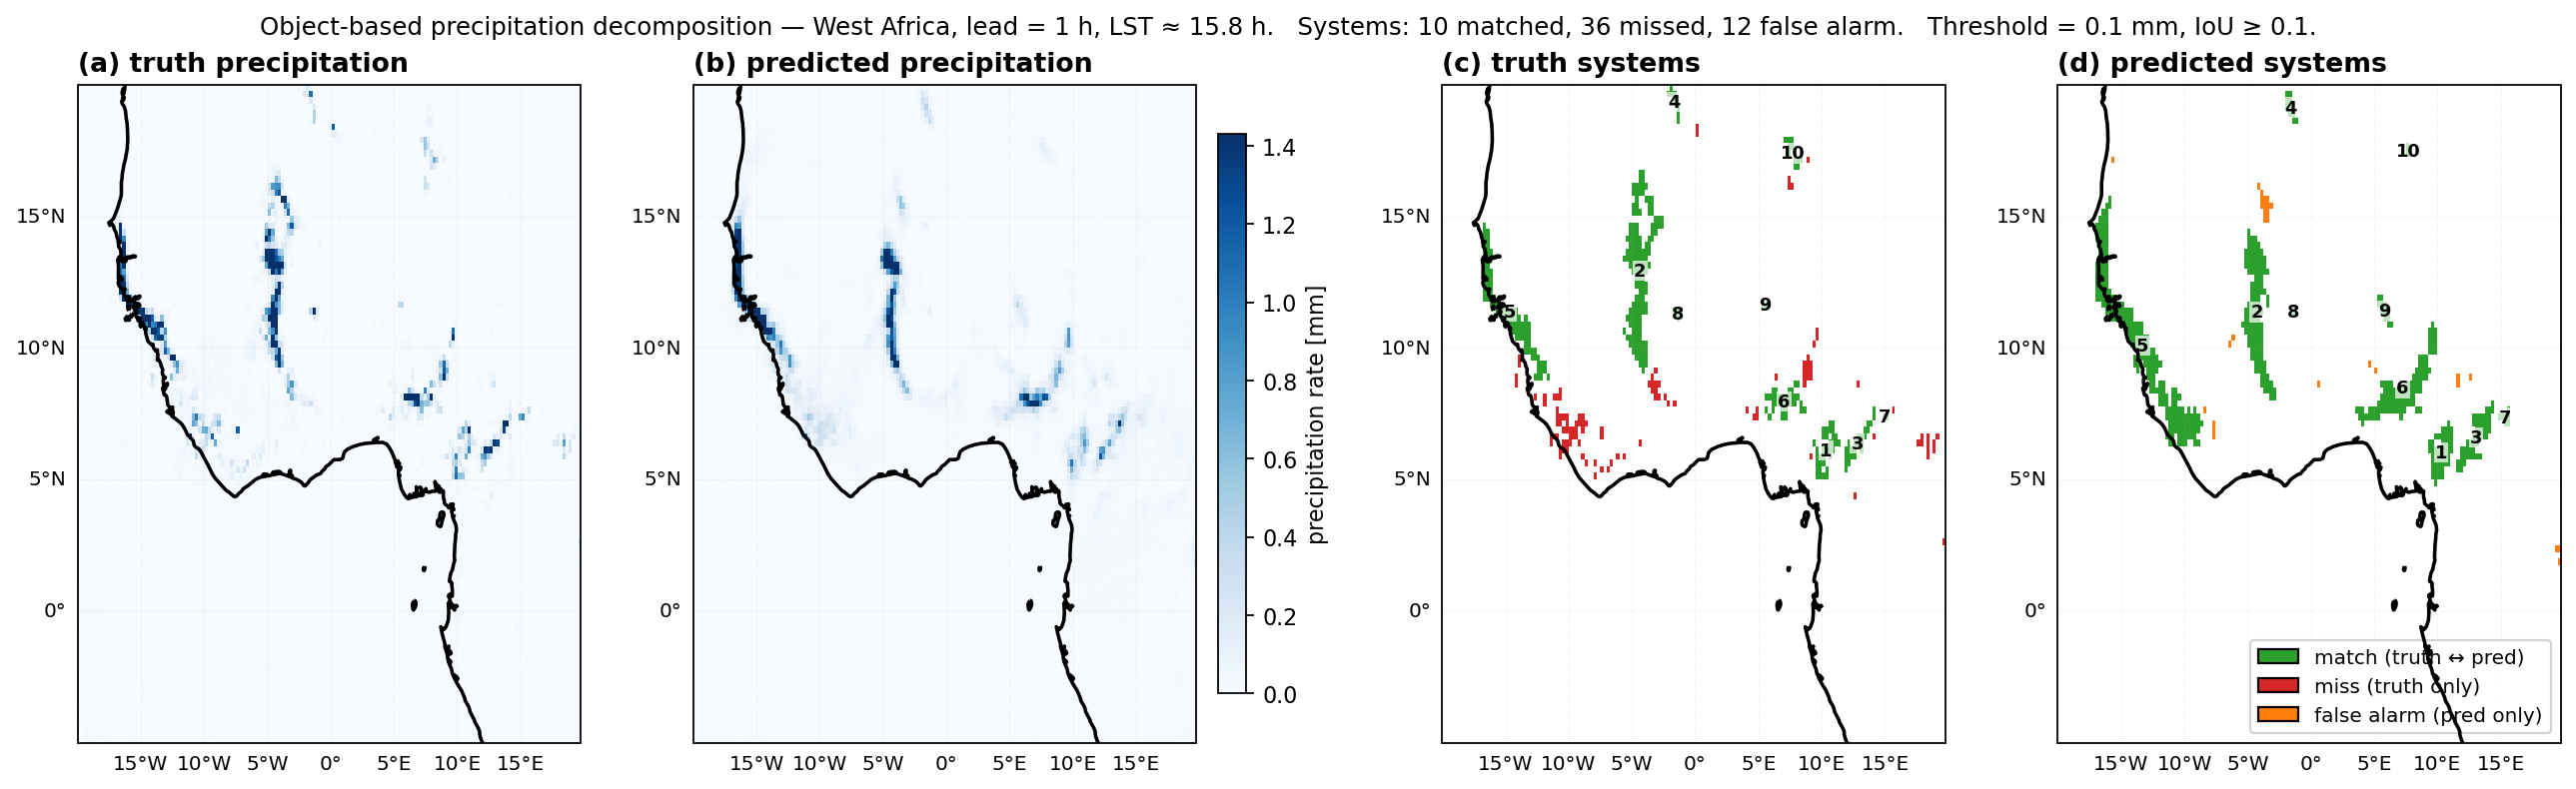
\includegraphics[width=\textwidth]{figures/method_illustration.png}
\caption{Object-based decomposition on one scene (West Africa, $1$\,h lead,
local solar time $\approx16$\,h). (a) truth precipitation; (b) prediction;
(c) truth systems coloured green\,=\,matched, red\,=\,missed; (d) predicted
systems coloured green\,=\,matched, orange\,=\,false alarm. The model captures
the large organised bands and misses the small ITCZ cells.}
\label{fig:method}
\end{figure}

\paragraph{Variable sensitivity.}
Figure~\ref{fig:confusion} compares the rain-rate contingency at leads $0$ and
$1$\,h for three input configurations.
At zero lead, the full nine-variable model (MSE + winds) substantially
outperforms the five-variable thermodynamics-only configurations: correlation
rises to $r=0.93$ from $r\approx0.87$ in both reduced sets, and the false-alarm
ratio drops from $0.31$--$0.36$ to $0.26$.
The improvement is attributable to the wind fields: dynamical convergence at
$500$ and $850$\,hPa provides direct information about where convection is
currently active, information not recoverable from thermodynamic scalars alone.
Replacing moist static energy with relative humidity at the same five-variable
count produces negligible difference, indicating that the thermodynamic form of
the moisture variable matters less than whether the dynamical fields are included.
The advantage of the nine-variable set narrows with lead time --- winds decouple
from future convective location faster than thermodynamic variables --- motivating
our focus on the nine-variable model as the best-case estimator.

\begin{figure}[t]
\centering
\begin{subfigure}{\textwidth}\centering
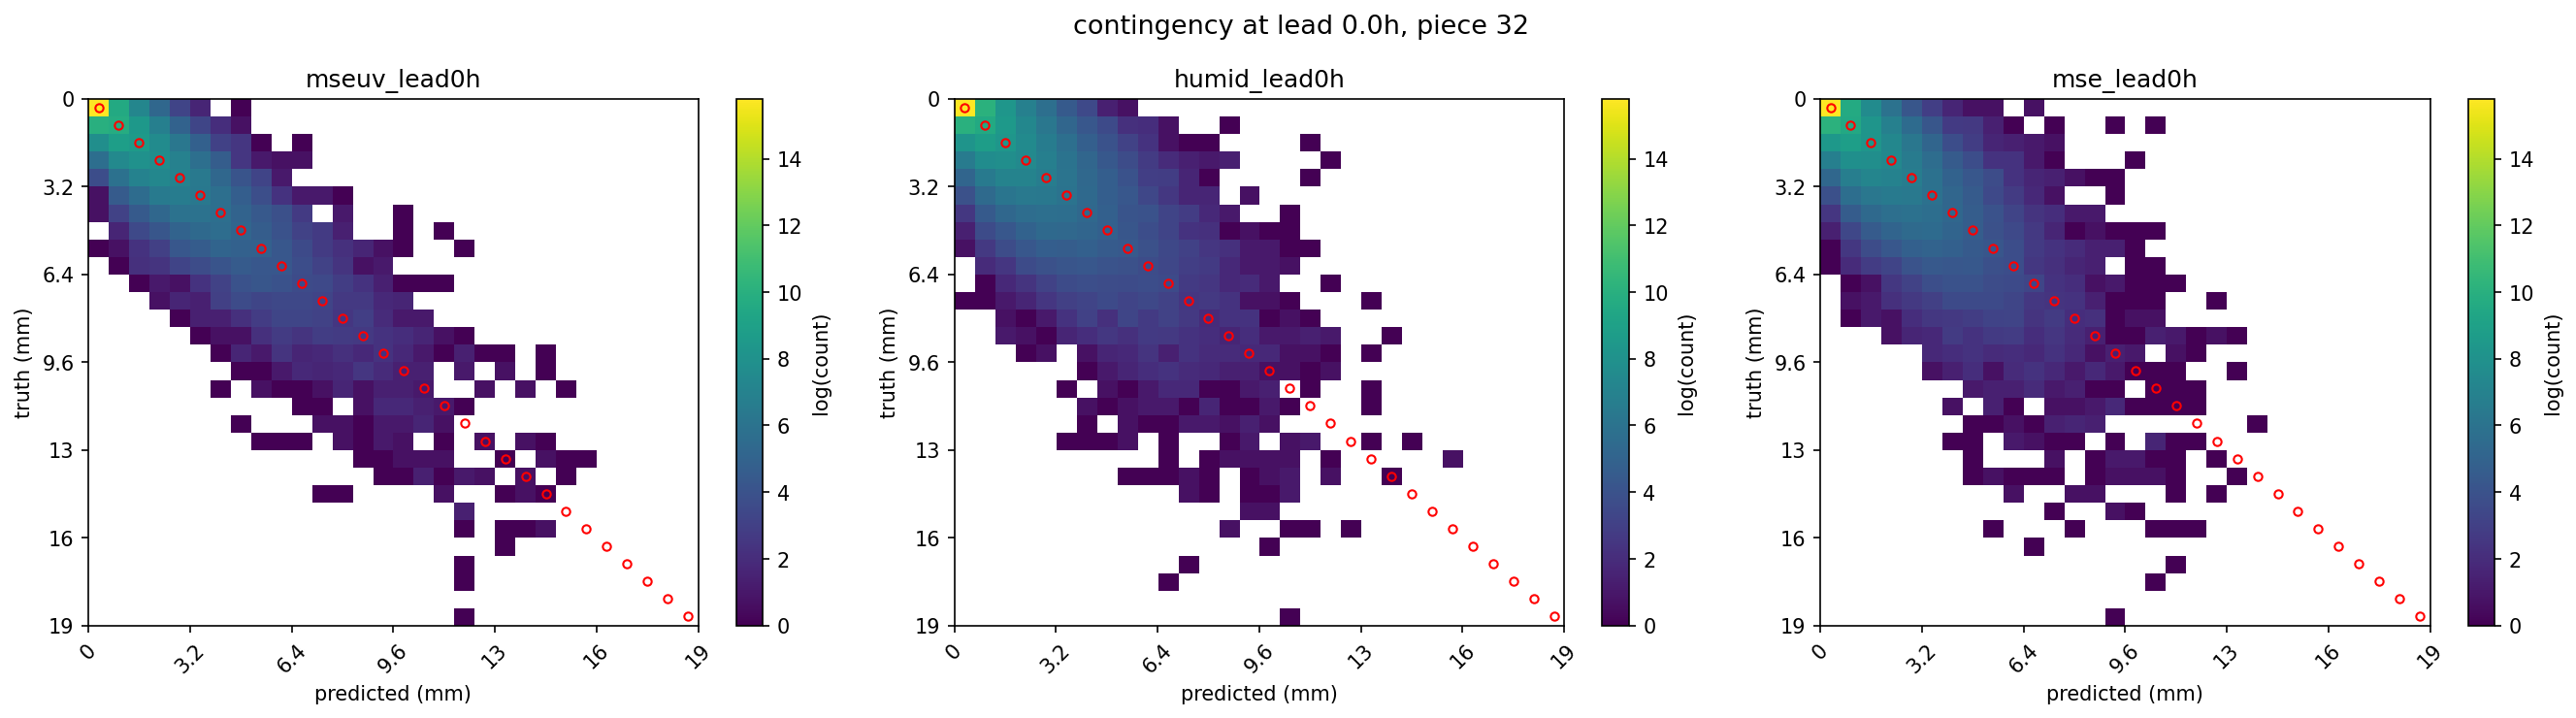
\includegraphics[width=\textwidth]{figures/contingency_compare_p32_lead0h.png}
\caption{lead $0$\,h}
\end{subfigure}\\[4pt]
\begin{subfigure}{\textwidth}\centering
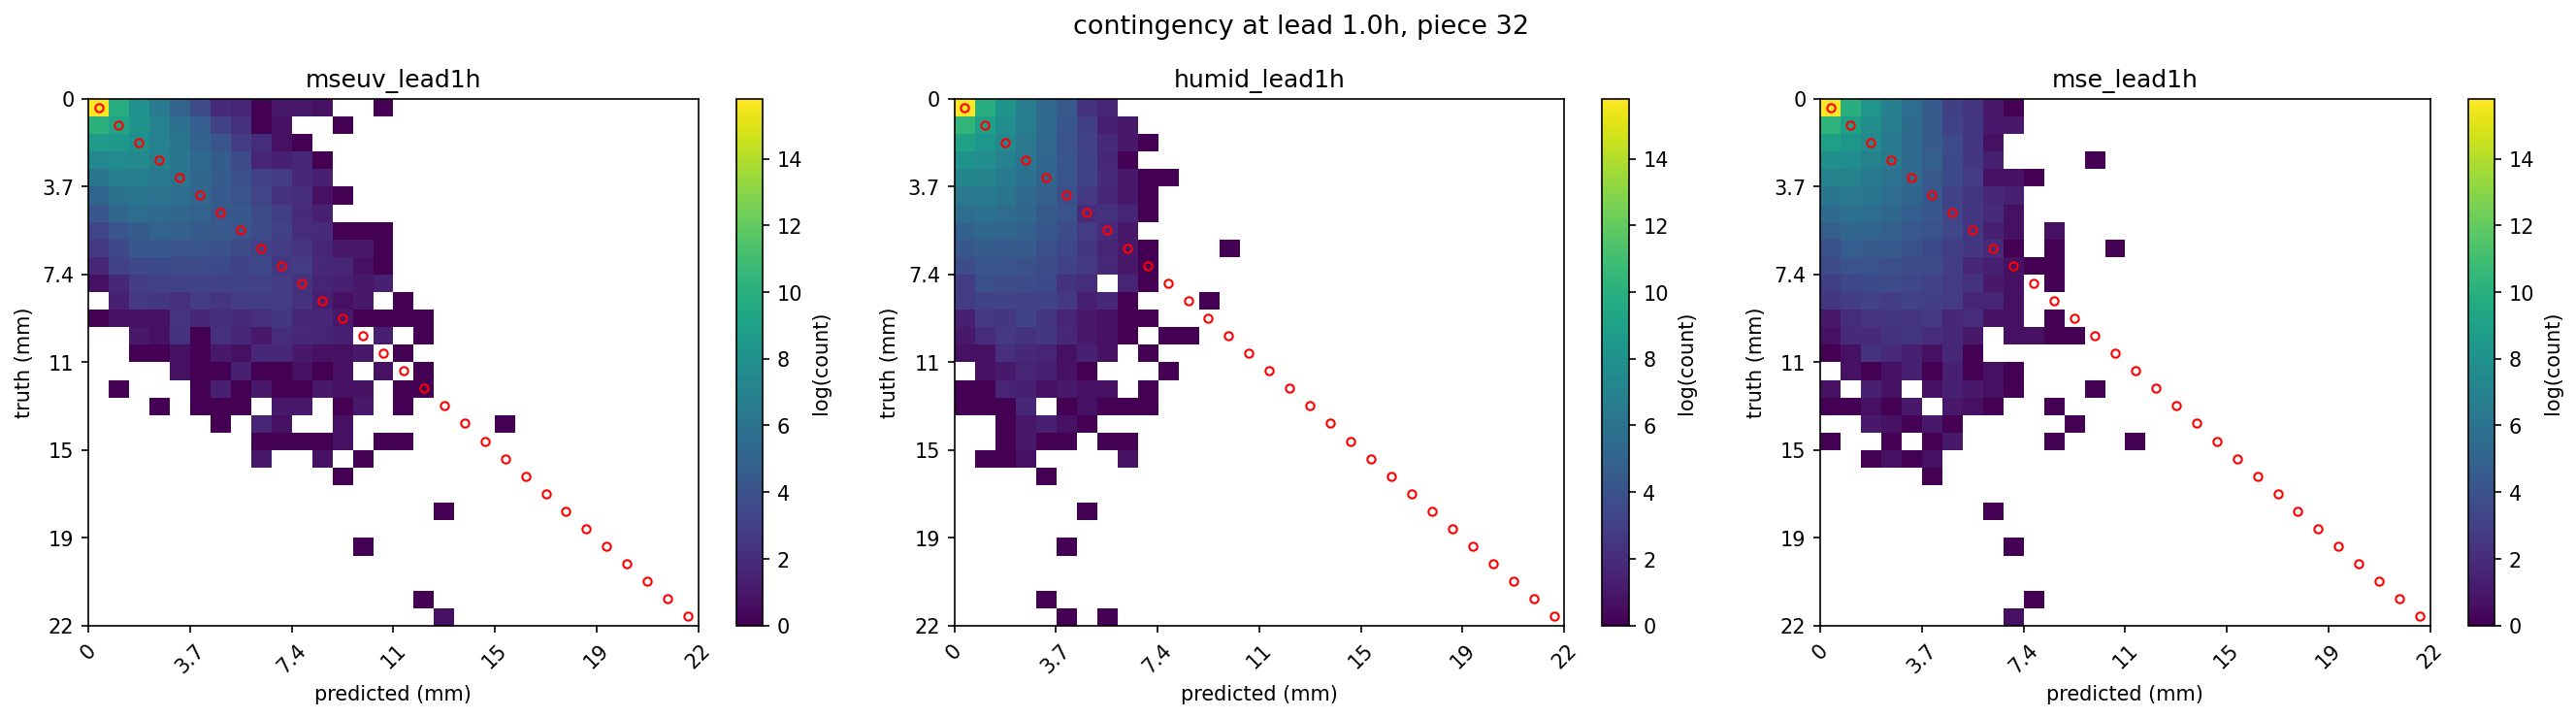
\includegraphics[width=\textwidth]{figures/contingency_compare_p32_lead1h.png}
\caption{lead $1$\,h}
\end{subfigure}
\caption{Rain-rate contingency (log counts) between truth ($y$) and prediction
($x$) at lead $0$\,h (top) and $1$\,h (bottom) for three input configurations
(\textsf{9var}: MSE + winds; \textsf{5var-mse}: MSE only; \textsf{5var-relhum}:
relative humidity only). Mass below the diagonal indicates intensity
under-prediction. Adding winds substantially reduces false alarms and improves
intensity estimation at zero lead.}
\label{fig:confusion}
\end{figure}

\subsection{Scale-dependent predictability horizon}
\label{sec:horizon}

The full scale decomposition at $3$\,h lead (Fig.~\ref{fig:scale}) reveals
how severely detection skill depends on system size.
Probability of detection rises monotonically from near zero for the smallest
systems ($L<65$\,km) to near unity for the largest ($L>200$\,km); the
false-alarm ratio mirrors it.
For matched systems, predicted objects are systematically too large
($\Delta\ln A>0$) and too weak ($\Delta\ln\rho<0$); at small scales the
precipitation budget is dominated by the detection term (missed precipitation),
not by distortion of correctly placed systems.

\begin{figure}[t]
\centering
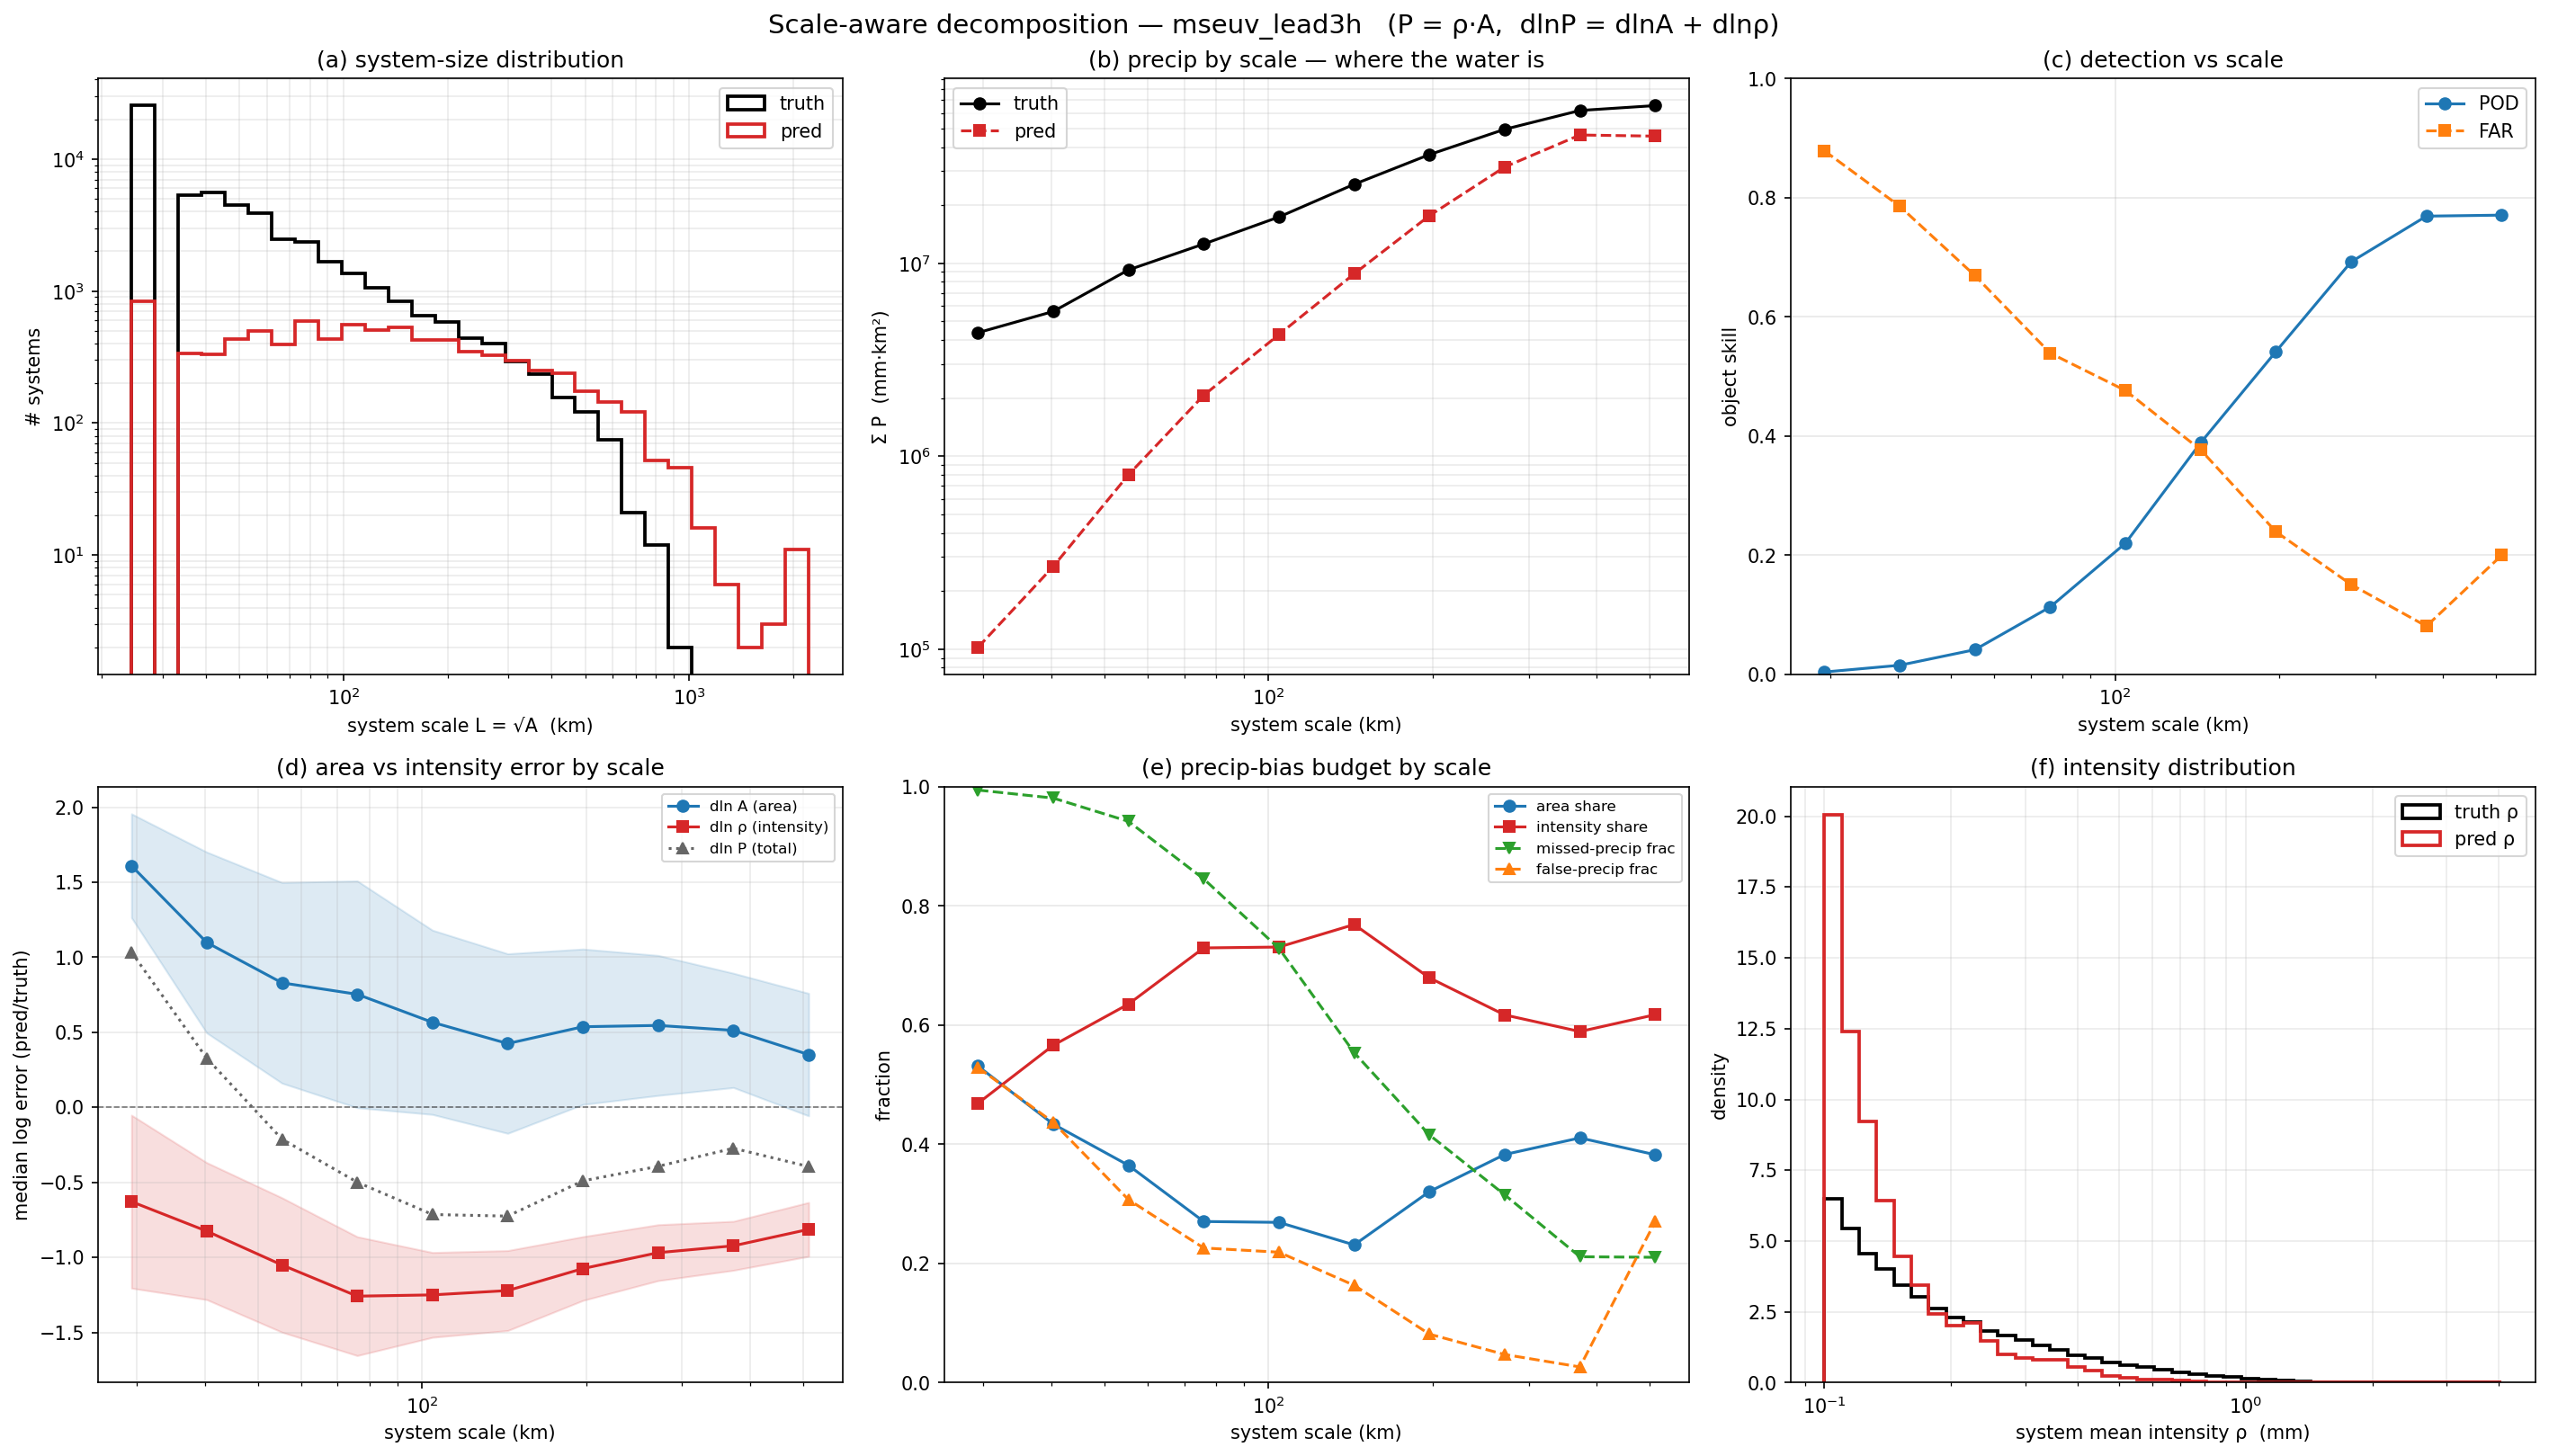
\includegraphics[width=\textwidth]{figures/scale_decomp_mseuv_lead3h_v2.png}
\caption{Scale-aware decomposition for the nine-variable model at $3$\,h lead.
(a) system-size distribution, truth vs prediction; (b) precipitation carried
by each scale; (c) POD and FAR vs scale; (d) median area ($\Delta\ln A$) and
intensity ($\Delta\ln\rho$) bias vs scale; (e) precipitation-bias budget
(area vs intensity share, plus missed/spurious fractions); (f) intensity
distribution. Detection of small systems is near zero; their error budget is
dominated by missed precipitation, not by distortion of correctly located
systems.}
\label{fig:scale}
\end{figure}

The collapse with lead is exponential and strongly scale-dependent
(Fig.~\ref{fig:horizon}, Table~\ref{tab:Te}).
For the trigger (detection), $T_e$ rises from $0.73$\,h for small systems
($L<65$\,km) to $8.8$\,h for large systems ($L>200$\,km) --- a factor of
twelve. Small convective initiation is forgotten by the resolved state in
under an hour; large organised systems remain locatable for nearly a day.

For the amplitude (intensity), the picture is more nuanced.
Large systems retain informative intensity prediction far beyond the $6$\,h
window ($T_e\!\approx\!21$\,h): once a large system is correctly located, its
predicted intensity is constrained by the slowly evolving large-scale
thermodynamic environment.
Small systems, however, lose amplitude skill at nearly the same rate as they
lose trigger skill ($T_e\!\approx\!0.91$\,h), because small-cell intensity is
sensitive to the same sub-grid boundary-layer fluctuations that govern whether
the cell fires at all.
The trigger/amplitude distinction in predictability therefore applies primarily
to large systems; for convective-scale objects, both trigger and amplitude are
effectively unpredictable beyond $\sim$1\,h.

The aggregate (all-scale) curves in Fig.~\ref{fig:horizon} reflect an
important asymmetry in how scales are weighted by each metric.
Trigger skill (POD) is count-weighted: small systems vastly outnumber large
ones, so the all-scale POD is dominated by the many missed small cells and
closely tracks the small-scale curve.
Amplitude skill is instead computed only over \emph{matched} systems; because
small systems are rarely matched (their POD is near zero), the matched pool is
dominated by the large systems that are successfully located, pulling the
all-scale intensity curve toward the large-scale result.
The aggregate numbers in Table~\ref{tab:Te} should therefore be read as:
trigger skill is effectively the worst case (small-system performance), while
aggregate amplitude skill reflects the best case (large-system performance).

The trigger $e$-folding time $T_e^{\text{det}}\!\sim\!0.7$\,h at convective
scales is an upper bound set by the atmosphere: it measures how fast the
resolved state loses predictive information about where the next cell fires,
regardless of forecast architecture.

\begin{figure}[t]
\centering
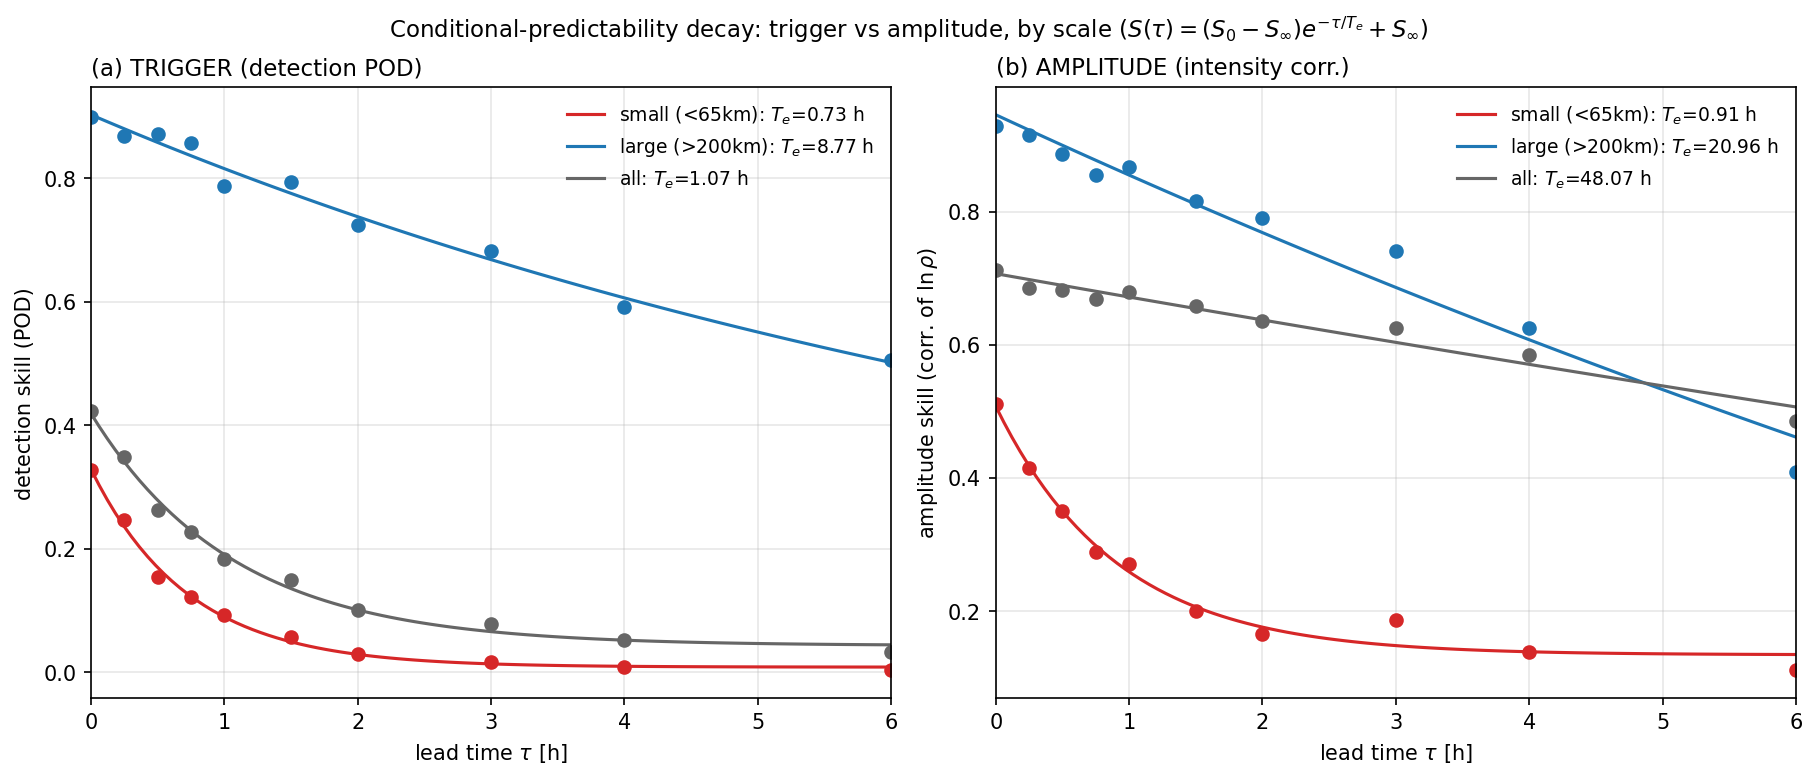
\includegraphics[width=\textwidth]{figures/predictability_horizon.png}
\caption{Predictive-information decay vs lead, by scale and component.
(a) Detection skill (POD) and (b) intensity skill (correlation of $\ln\rho$
for matched systems), with exponential fits (Eq.~\ref{eq:efold}).
The all-scale trigger curve tracks the small-scale curve because POD is
count-weighted and small cells dominate the system population; the all-scale
amplitude curve tracks the large-scale curve because the matched pool (on which
intensity is evaluated) is dominated by the large systems that are successfully
detected.
Trigger skill for small systems ($T_e^{\text{det}}\!=\!0.73$\,h) is a factor
of twelve shorter than for large systems ($T_e^{\text{det}}\!=\!8.8$\,h).
Amplitude of large systems persists well beyond 6\,h
($T_e^{\text{int}}\!\approx\!21$\,h), while small-system amplitude fades at
a similar rate to the trigger ($T_e^{\text{int}}\!=\!0.91$\,h).}
\label{fig:horizon}
\end{figure}

\begin{table}[t]
\centering
\caption{Fitted predictability parameters (Eq.~\ref{eq:efold}): zero-lead
skill $S_0$, $e$-folding time $T_e$, and climatological floor $S_\infty$.
Large-system intensity $T_e$ exceeds the $6$\,h window and is poorly
constrained (denoted $\gg6$).}
\label{tab:Te}
\begin{tabular}{llccc}
\hline
band & term & $S_0$ & $T_e$ [h] & $S_\infty$ \\
\hline
small ($<65$\,km)  & detection & 0.33 & \textbf{0.73} & 0.01 \\
small ($<65$\,km)  & intensity & 0.51 & 0.91          & 0.13 \\
large ($>200$\,km) & detection & 0.90 & \textbf{8.77} & 0.09 \\
large ($>200$\,km) & intensity & 0.95 & $\gg6$        & ---  \\
all                & detection & 0.42 & 1.07          & 0.04 \\
all                & intensity & 0.71 & $\gg6$        & ---  \\
\hline
\end{tabular}
\end{table}

\subsection{Architecture independence: comparison with GraphCast}
\label{sec:graphcast}

The behaviour is not specific to our model or training data.
Applying the same object-based decomposition to GraphCast
\citep{lam2023graphcast} precipitation at $6$\,h lead (verified against ERA5,
with a rate-matched detection threshold of $0.4$\,mm\,h$^{-1}$) reproduces the
same signature (Fig.~\ref{fig:graphcast}): POD rises monotonically with scale
and small systems are essentially undetected.
GraphCast was trained on ERA5 reanalysis using a graph-neural-network
architecture with no shared design choices with our U-Net, verified against a
different truth (ERA5 vs MPAS), and evaluated at a different lead and
accumulation window ($6$\,h vs $15$\,min).
The robust, comparable quantity is the \emph{shape} of the scale-dependence
curve, not its absolute level; both models occupy the same scale-collapse
regime.
This indicates that ``large-system detector'' is a property of data-driven
precipitation forecasting at convective scales, not of any one network.

\begin{figure}[t]
\centering
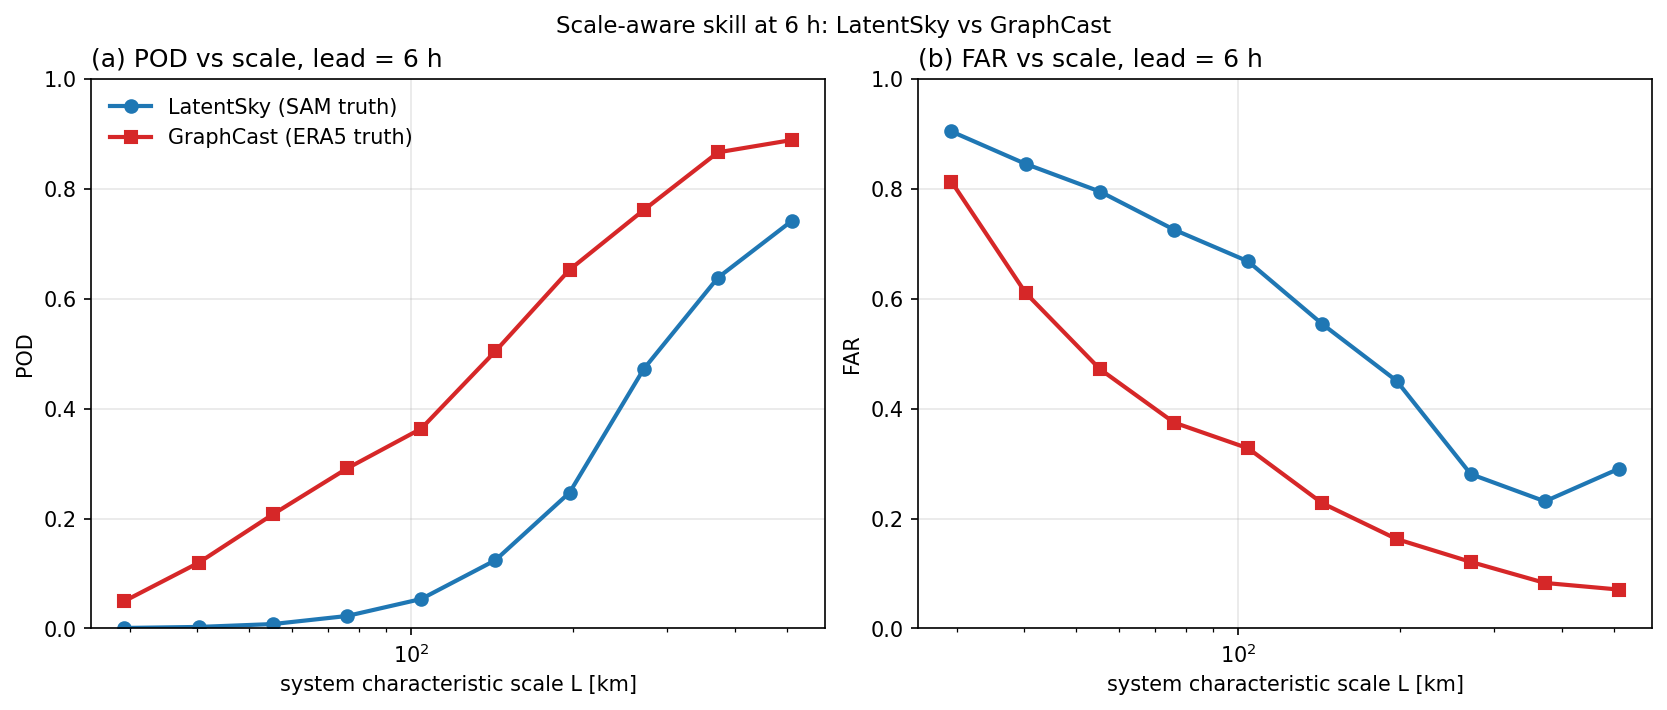
\includegraphics[width=\textwidth]{figures/graphcast_vs_latentsky_6h_ratematched.png}
\caption{POD (a) and FAR (b) vs system scale at $6$\,h lead for our model
(MPAS truth) and GraphCast (ERA5 truth), at a rate-matched detection threshold
($0.4$\,mm\,h$^{-1}$). Both show the monotonic scale-dependent detection
collapse. Absolute levels differ because of the different truths and
accumulation windows; the robust quantity is the shape of the curve.}
\label{fig:graphcast}
\end{figure}

\section{Discussion}
\label{sec:discussion}

\paragraph{Trigger vs amplitude: two regimes.}
Our results separate precipitation predictability into two physically distinct
components. The \emph{amplitude} --- how intense a system will be --- inherits
the slow memory of the large-scale thermodynamic environment (column water
vapour, CAPE, radiative forcing), which evolves on timescales of hours to days.
This is why large-system intensity remains informative far beyond the $6$\,h
window ($T_e\!\approx\!21$\,h). The \emph{trigger} --- whether and where a
cell fires --- is governed by sub-grid processes (boundary-layer thermals,
cold-pool collisions, mesoscale convergence features) that are effectively
stochastic at the resolved $0.25^\circ$ scale.
For small convective cells the two regimes collapse: trigger and amplitude
skills decay at comparable rates ($T_e\!\sim\!0.7$--$0.9$\,h), because
small-cell intensity is sensitive to the same sub-grid fluctuations that
determine whether initiation occurs at all.

\paragraph{The forced diurnal cycle: what survives the trigger horizon.}
Once the lead exceeds the trigger horizon, the only predictable component of
small-scale convection is the externally forced diurnal cycle.
Figure~\ref{fig:diurnal} shows that over land, detection of small systems (POD)
is phase-locked to the afternoon convective maximum, while over ocean detection
is flat in local solar time --- a pattern that persists across leads well beyond
$T_e$.
The model is not predicting rain from its inputs at long leads; it is
reinjecting a learned climatological prior.

The ablation experiment (Fig.~\ref{fig:ablation}) confirms this mechanism.
Replacing the solar-tied inputs ($T_{2m}$, low-level MSE, and OLR) with their
per-pixel daily means before inference removes the instantaneous phase signal
while preserving geographic structure. The predicted afternoon land peak
survives all ablations, showing the diurnal cycle is encoded in the model
weights rather than read from the instantaneous inputs.

This has a practical implication: standard pixel scores cannot distinguish
climatological reinjection from genuine forecast skill, because both produce
temporally correlated errors that inflate the apparent score.
The object decomposition can make this distinction: a model that substitutes
learned climatology for forecast skill produces detection skill that flattens
to the asymptotic floor $\mathcal{S}_\infty$, rather than continuing to decay,
and this floor is visible in Table~\ref{tab:Te}.
Whether the diurnal residual is read as a positive result (the forced component
of convection is correctly recovered) or a cautionary one (reported skill is
inflated by climatology) depends on the application; the decomposition makes
the distinction transparent in a way that pixel scores cannot.

\begin{figure}[t]
\centering
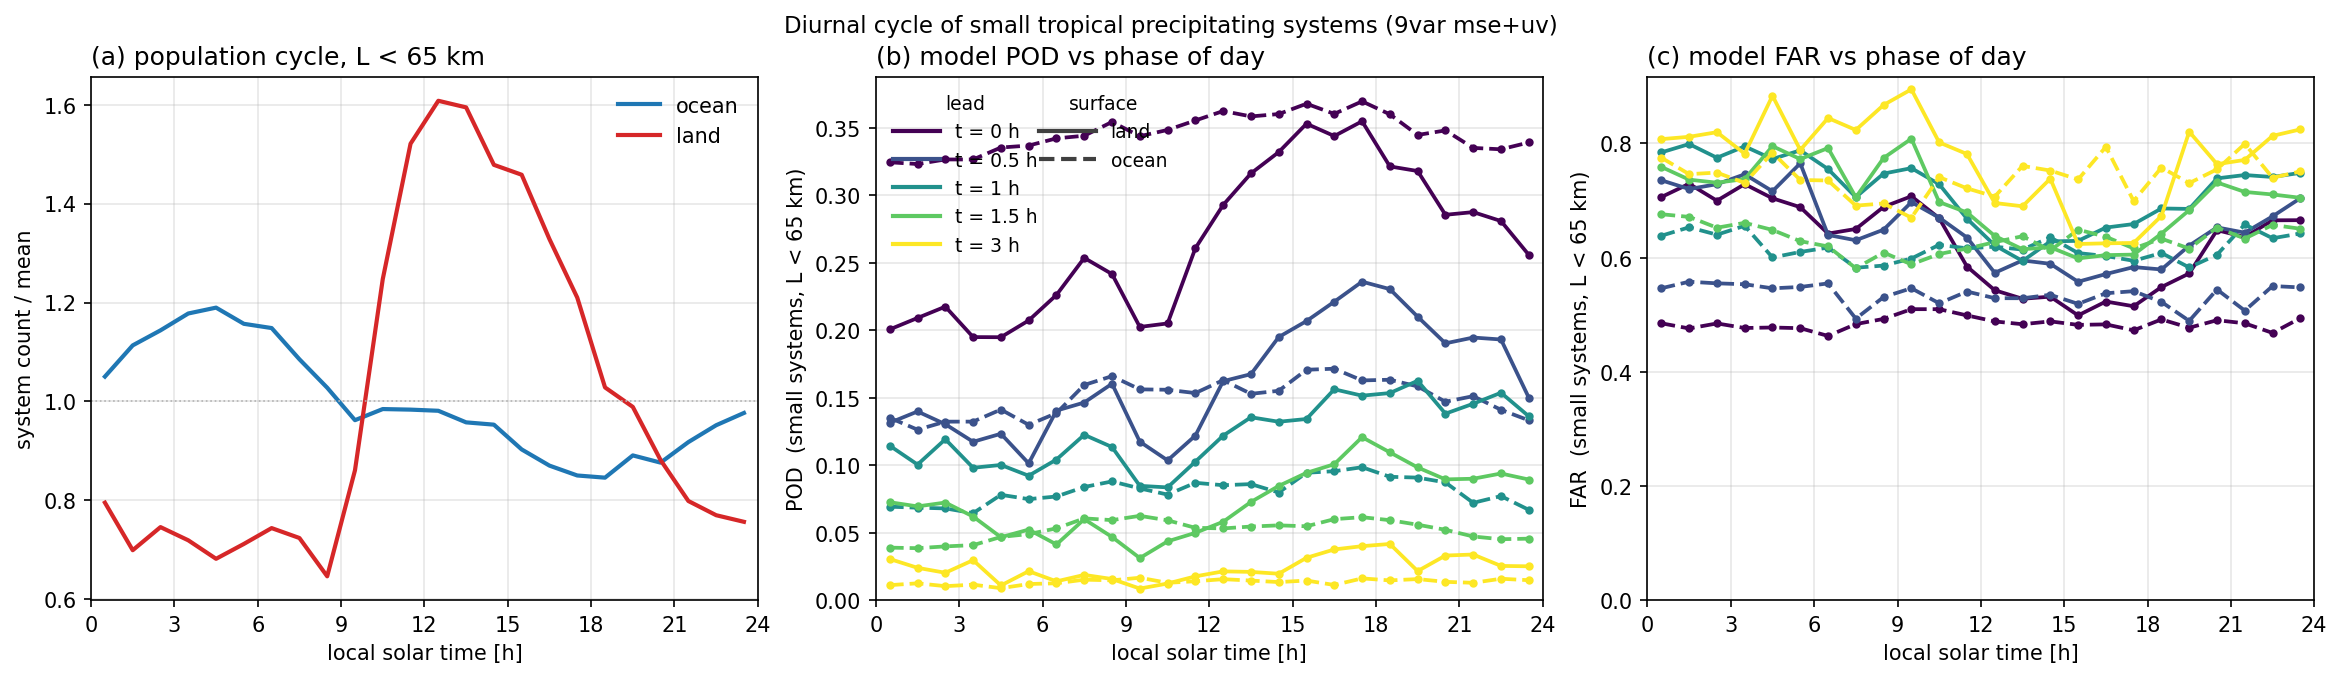
\includegraphics[width=\textwidth]{figures/diurnal_small_systems.png}
\caption{Diurnal cycle of small ($L<65$\,km) precipitating systems.
(a) truth population cycle vs local solar time, land vs ocean;
(b) model POD vs local solar time at several leads, land (solid) vs ocean
(dashed). Land detection is phase-locked to the afternoon convective maximum;
ocean detection is flat.}
\label{fig:diurnal}
\end{figure}

\begin{figure}[t]
\centering
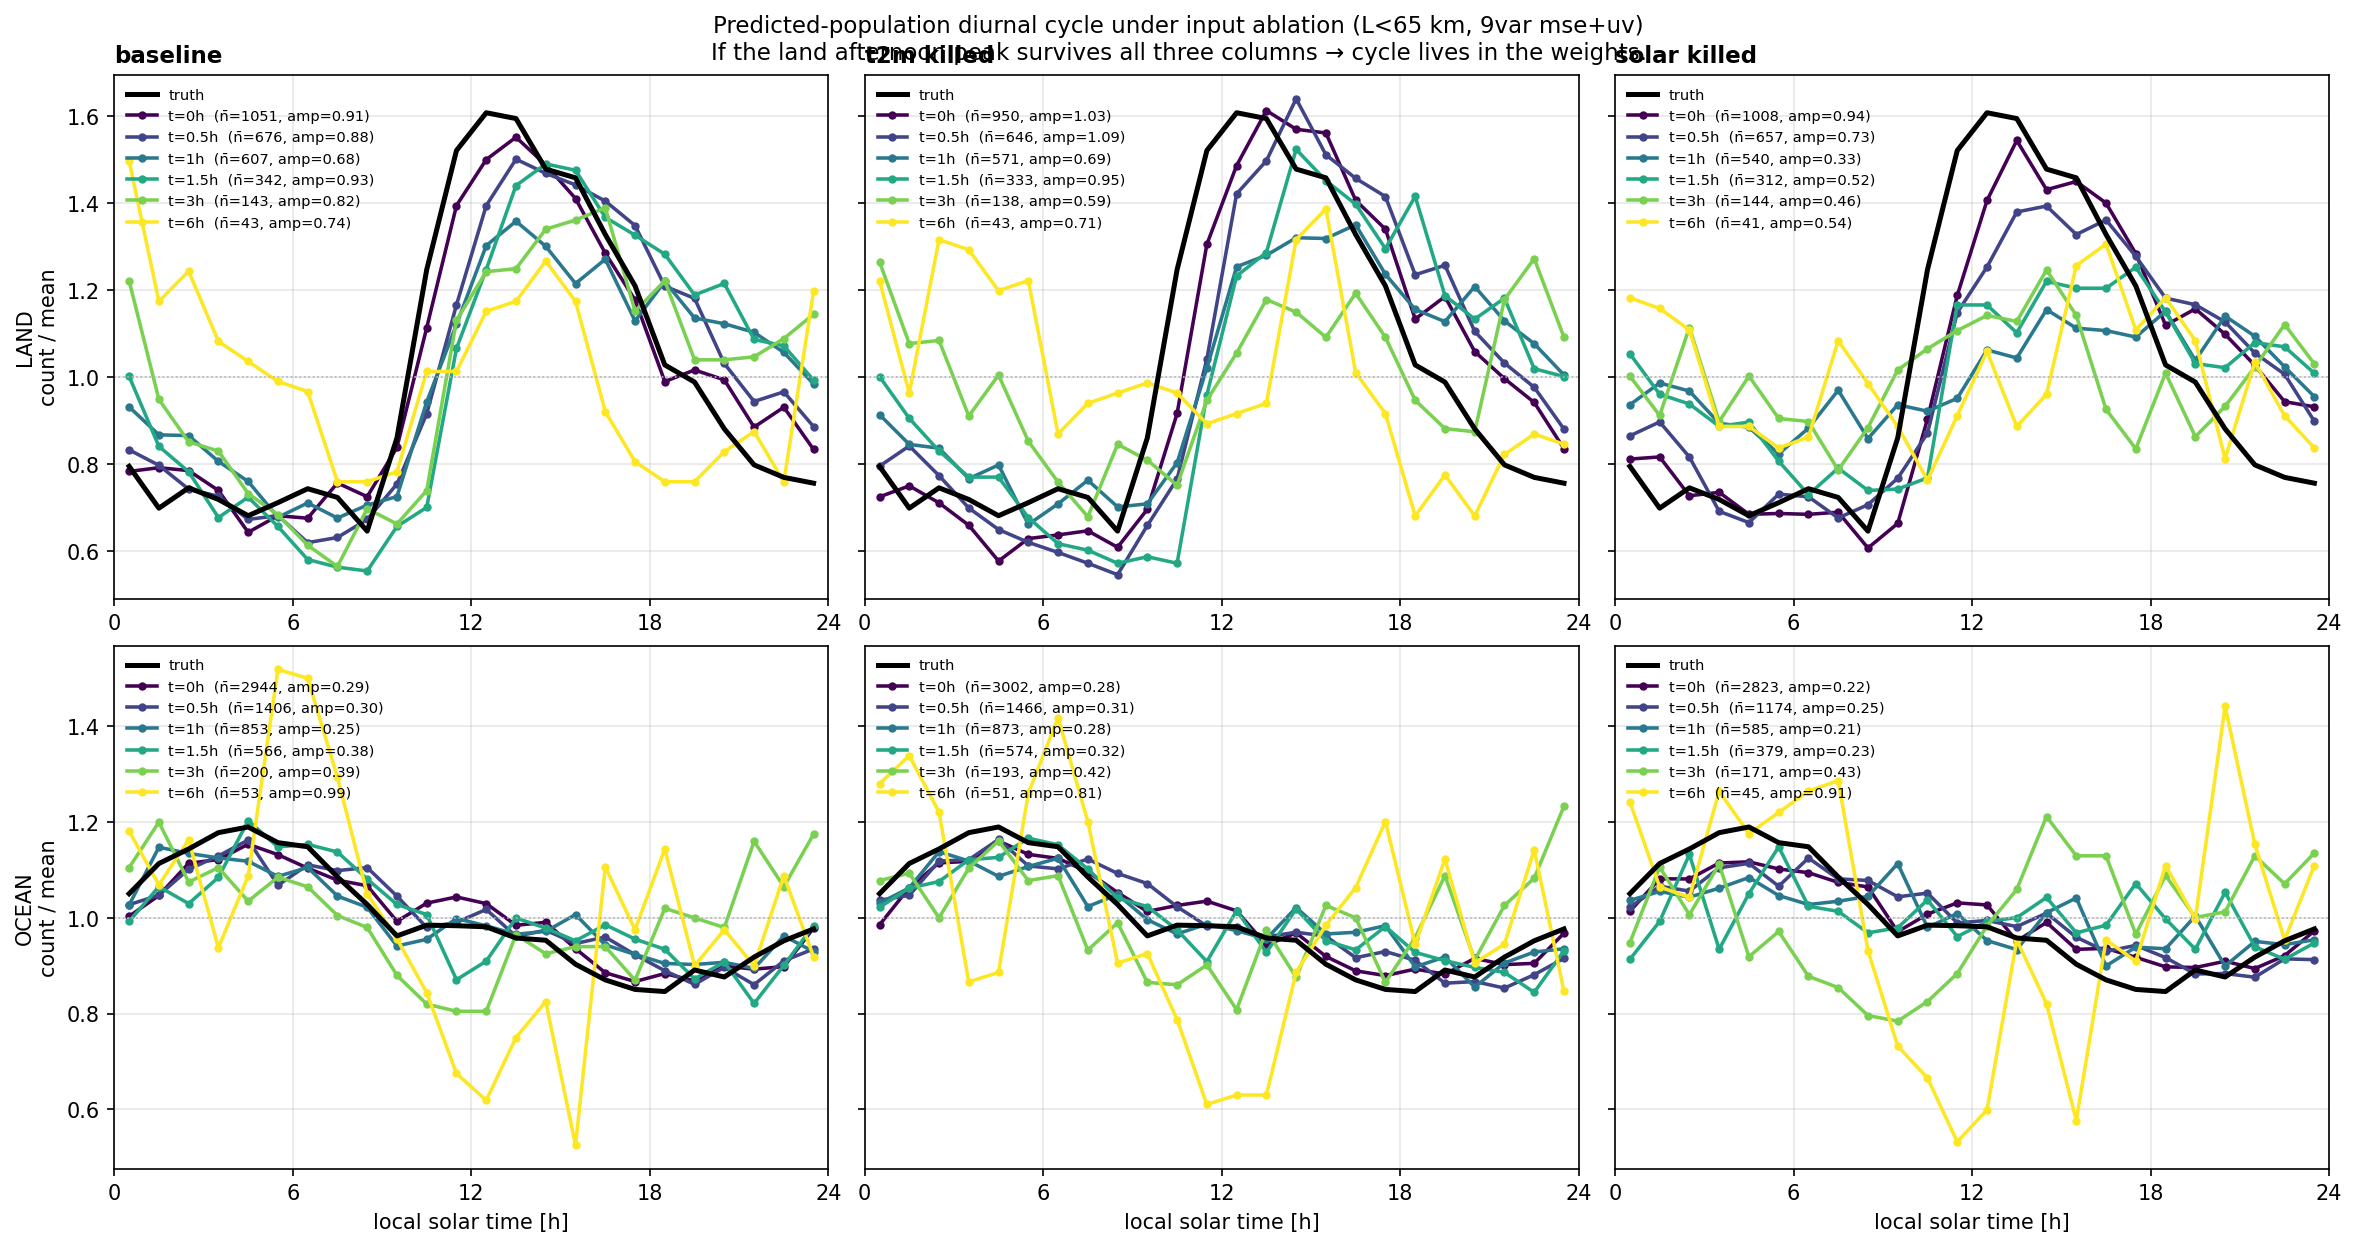
\includegraphics[width=\textwidth]{figures/diurnal_ablation_predicted_cycle.png}
\caption{Input-ablation test. Predicted small-system population cycle vs local
solar time (top: land, bottom: ocean) for the baseline and two ablations in
which solar-tied inputs are replaced by their daily mean. The land afternoon
peak survives all ablations, showing the diurnal cycle is encoded in the model
weights.}
\label{fig:ablation}
\end{figure}

\paragraph{Implications for AI precipitation forecasting.}
The convective-scale trigger horizon $T_e\!\sim\!0.7$\,h is set by the
atmosphere, not by the model: no improvement to the state-evolution core of
a deterministic system --- better architecture, more training data, higher
spatial resolution --- can cross it, because the limit lies in the predictive
information content of the resolved state itself.
That GraphCast shows the same scale-dependent collapse is consistent with this
bound being physical rather than architectural.
Below the horizon, the conditional distribution of precipitation is genuinely
broad; the only routes to better small-scale forecasts are (i)
\emph{stochastic} outputs that sample the conditional distribution rather than
predict its blurred mean \citep{ravuri2021}, and (ii) new predictors carrying
sub-grid trigger information (dense surface observations, lightning, radar).
The smoothing bias we observe --- predicted systems too large and too weak ---
is exactly what a deterministic model minimising MSE against an unpredictable
target should produce.

\paragraph{Limitations.}
The analysis uses a single 40-day boreal-winter MPAS simulation; MPAS
overestimates heavy convective rainfall relative to IMERG, and ``resolved''
is defined by the $0.25^\circ$ coarsening, so the trigger horizon is
conditional on that scale and on the nine-variable state used here.
The GraphCast comparison mixes truth sources (MPAS vs ERA5) and accumulation
windows ($15$\,min vs $6$\,h); the robust statement is the shape of the scale
dependence, not absolute skill levels.
Natural next steps are an identical-twin intrinsic-predictability comparison,
verification against IMERG observations, and a generative model to test whether
sampling the conditional distribution recovers the small-scale rain that a
deterministic network smooths away.

\section{Conclusion}
\label{sec:conclusion}

Resolution does not equal predictability.
Using a global convection-permitting simulation as truth and per-lead neural
networks as best-case state-to-rain estimators, we have measured how much
predictive information the resolved large-scale environment carries about
precipitation, how fast that information fades with lead, and whether the
result is specific to one model.

For the trigger (detection), predictability $e$-folds in $0.73$\,h at
convective scales ($L<65$\,km) and in $8.8$\,h for large organised systems
($L>200$\,km) --- a factor of twelve.
For the amplitude (intensity), large systems remain predictable far beyond the
$6$\,h window, while small systems lose amplitude skill as rapidly as they lose
trigger skill.
Past the trigger horizon, the only surviving small-scale signal is the
externally forced diurnal cycle, which the network encodes as a learned
climatological prior and reinjects regardless of the instantaneous inputs;
the object-based decomposition reveals this substitution where pixel scores
cannot.
The same scale-dependent detection collapse appears in GraphCast, indicating a
physical, architecture-independent bound on data-driven precipitation
forecasting at convective scales.

For the design of AI precipitation systems, the implication is clear:
deterministic minimisation of MSE cannot close the convective gap.
Stochastic outputs and new sub-grid predictors are the two routes beyond the
predictability horizon set by the resolved state.

\paragraph{Acknowledgements.}
[To be completed: funding sources; NCAR Derecho/Casper computing allocation;
DYAMOND data access via DKRZ.]

\paragraph{Data availability.}
The DYAMOND MPAS simulation is available through the DKRZ long-term archive.
ERA5 reanalysis is available through the Copernicus Climate Change Service.
GraphCast outputs were produced following \citet{lam2023graphcast}.

\paragraph{Code availability.}
Code for the LatentSky network and the object-based decomposition will be
released upon acceptance at [repository URL to be provided].

\printbibliography

\end{document}
